
\documentclass[11pt]{article} %This sets the font size and the document class of your report. In this case we use 'article' as that is ideal for shorter reports. 

\usepackage[top=2.54cm, bottom=2.54cm, left=2.75cm, right=2.75cm]{geometry} %This sets the margins of the report.
\usepackage{graphicx} % A package allowing insertion of images into the text.
\usepackage{subcaption}
\usepackage{caption}

\usepackage{cite}         % A package that creates references in the IEEE style. 
\newcommand{\citet}{\cite} % Use with cite only, so that it understands the natbib-specific \citet command
\bibliographystyle{ieeetr} % IEEE referencing (use in conjunction with the cite package)

%% Author-date style citation:
%\usepackage[round]{natbib} % A package that creates references in the author-date style, with round brackets
%\renewcommand{\cite}{\citep} % For use with natbib only: comment out for the cite package.
%\bibliographystyle{plainnat} % Author-date referencing (use in conjunction with the natbib package)

\usepackage{listings}
\usepackage{xcolor}
\lstset{
	language=C++,
	basicstyle=\ttfamily\small,
	keywordstyle=\color{blue},
	commentstyle=\color{gray},
	stringstyle=\color{red},
	numbers=left,
	captionpos=b
}

\usepackage{color} % Allows the colour of the font to be changed by using the '\color' command: This is just to support the blue comments in this template...use standard (black) text in your report.

\linespread{1.2} % Sets the spacing between lines of text.
\setlength{\parindent}{0cm}  % Suppresses indentation of text at the start of a paragraph

\begin{document} % This begins the document proper and ends the pre-amble
\begin{titlepage} % Begins the titlepage of the document
\begin{center} % Starts the beginning of an environment where all text is centered.

{\Huge Simulating a Particle Detector and Particle Decay in C++ }\\[0.5cm] % [0.5cm] sets the distance between this line and the next.
\textit{Aidan Hughes}~\\[0.3cm] % The '\\' starts a new paragraph, and will only work after a paragraph has started, unless we use '~'.
\textit{11306492}~\\[0.3cm]
School of Physics and Astronomy~\\[0.3cm]
University of Manchester~\\[0.3cm]
Third Year Code Report~\\[0.3cm]
May 2026~\\[2cm]



\end{center}
{\textbf{Abstract}}~\\[0.3cm]
The aim of this project was to utilize object oriented programming practices to create a particle detector and particle decay simulators in C++. It consists of two main inheritance chains, one for the particle classes and another for sub-detector classes. These classes, and their respective container classes ParticleBunch and Detector, practice encapsulation by storing data members as private or protected with access via public member functions. The use of virtual and pure virtual functions in the abstract parent classes of the hierarchy enables polymorphism in the child classes. 
\end{titlepage}
\pagenumbering{gobble} % This stops the title page being numbered
\clearpage
\pagenumbering{arabic} % sets the style of page numbering for the report
\setcounter{page}{2} % Starts the numbering at page 2 as typically the first page is not numbered

\newpage % Starts a new page to begin the report on.

\section{Introduction} 
\label{intro}
The aim of this project was to create a C++ library that simulates a particle detector and its detecting functionality through the use of object oriented programming. As an addition, this code also aims to simulate particle decays within an accelerator. Particle detectors, such as ATLAS or the CMS, compose of multiple sub-detector types, each of which measure different types of particles. 

The tracker, the first sub-detector a particle will pass through, uses magnetic fields to measure particle paths, so can only measure charged particles. Next are the calorimeters, which are split into two, an electromagnetic and a hadronic calorimeter. The electromagnetic calorimeter causes electrons and photons to trigger a particle shower which is measured to finds their energy. The hadronic calorimeter does the same but for protons and neutrons. Finally, due to muons high energy, they are not turned into showers by the calorimeters, and pass through to the Muon Spectrometer sub-detector. Using information about which sub-detectors were triggered, the type of particle that passed through can be deduced. These sub-detectors also have a detection efficiency associated with them, which compares the number of particles detected to the number produced during an event, usually represented as a percentage. 

Along with the particles mentioned above, tau and Higgs particles are also found in accelerators, but decay quickly to other particles. This project focuses on the decays to muon and neutrinos for tau and di-photon decay for the Higgs. All particles have a four-momentum, which is a relativistically conserved property, akin to conservation of three-momentum in classical mechanics. Many particles also have masses, charges or even type specific conservation numbers like lepton number. 

To simulate the sub-detectors and particles in C++, an inheritance chain was established for each. 
\section{Code Implementation}
Object oriented programming (OOP) is built on four pillars: encapsulation, inheritance, polymorphism and abstraction.
\subsection{FourMomentum} 

The FourMomentum class is constructed from 4 doubles corresponding to each four-momentum component: energy and the x, y and z momenta.
The four-momentum components were stored as private double member variables within the FourMomentum class, as this is a more readable format then a vector in which the index corresponding to each property is not explicit to anyone extending the class.
The components are accessed via getters and setters, returning the value as a double, and the setters taking a double as input and changing the member variable. Using getters and setters along with private variables is an example of encapsulation. In this case the encapsulation allowed for value checking on inputted energy, Listing \ref{ssss}, to ensure it was positive, throwing an error if not, which would not have been possible if the data member was publicly accessible.

\begin{lstlisting}[firstnumber=30, caption={Showing setter for energy private data member in FourMomentum.cpp.}, label=ssss]
// Setter
void FourMomentum::set_energy(double energy)
{
  if(!validate_energy(energy))
  {
    throw std::invalid_argument("negative energy");
  }
  energy_ = energy;
}
\end{lstlisting} 

A major benefit of constructing separate class to hold particle four momentum is to be able to overload operators, such as the addition (+) and increment (+=) operators shown in Listing \ref{fmoperator}, to provide functions more suitable to the class. The addition operator now adds two four-momenta component-wise and returns the result as a new FourMomentum object, acting as a form of static (compile-time) polymorphism. The advantage of this can be seen in the overloaded increment operator, where the addition operator is used to add the second FourMomentum object's components into the first's, utilizing the 'this' pointer, which always points to the calling object. 

\begin{lstlisting}[firstnumber=39, caption={Code snippet from FourMomentum.cpp showing the overloading of + and += operators to add FourMomentum objects component-wise.}, label=fmoperator]
// Addition
FourMomentum FourMomentum::operator+(const FourMomentum &vector) const
{
  FourMomentum result(energy_ + vector.energy_, x_momentum_ 
    + vector.x_momentum_, y_momentum_ + vector.y_momentum_,
		 z_momentum_ + vector.z_momentum_);
  return result;
}
// Increment
FourMomentum & FourMomentum::operator+=(const FourMomentum &vector)
{
  *this = *this + vector;
  return *this;
}
\end{lstlisting} 

Listing \ref{fmoperator} also showcases the use of const and references, used widely in this project. First, the FourMomentum object, vector, is passed to the function as a const reference, which means a copy of memory address of the vector is passed to the function, rather than a copy of the object. This saves on memory usage as objects are much larger than their addresses, so take up more memory when copied. However, referencing allows the underlying object to be changed by the function, which is not wanted for the addition and increment operators, so const is used, which ensures the object is not changed by the function using it. Moreover, the addition operator is defined as a const member function by the const at the end of line 40, which prevents it from changing the calling FourMomentum object. This is not included in the increment operator as that intents to change the calling FourMomentum, instead the return is a reference to the calling FourMomentum. 

The FourMomentum class also includes dot product and info member functions, which return the dot product as a double or print the components of the FourMomentum. 

\subsection{Particle}

The Particle class is constructed using a FourMomentum object, a double for mass and a integer for charge. The FourMomentum is stored as a unique pointer to the FourMomentum object, as this means only the address to the FourMomentum stored in the Particle. A smart pointer will protect against memory leaks by deleting the object and itself when it goes out of scope, unlike a raw pointer. The unique kind was chosen as only the particle can possess its own four momentum, so there is no need for other pointers to the FourMomentum, and therefore no need for a shared pointer. 

A consequence of using smart pointers is the need to use the Rule of 5, that being the redefinition of the copy constructor and assignment, Listing 
\ref{ruleof5}, and the move constructor and assignment, for which the default was sufficient. The copy  had to be constructor and assignment redefined as unique pointers cannot be copied or a new unique pointer made pointing to the same FourMomentum object as that would result in two unique pointers to the same object, which is not allowed as would result in the first pointer deleting itself and the object when out of scope, leaving the second pointing to nothing, therefore allowing memory leaks. So instead, a copy of the FourMomentum is made for the new (or existing for assignment) pointer to point to. The default move constructor and assignment can still used however, as moving a unique pointer does not cause two pointers to the object. 

\begin{lstlisting}[firstnumber=39, caption={Code snippet from Particle.cpp showing the copy constructor and assignment redefinition in the Particle class.}, label=ruleof5]
// Copy Constructor
Particle::Particle(const Particle &other_particle) : four_momentum_ptr_ 
(std::make_unique<FourMomentum>(*other_particle.four_momentum_ptr_)),
mass_(other_particle.mass_), charge_(other_particle.charge_){}
// Copy Assignment
Particle & Particle::operator=(const Particle &other_particle)
{
  if(&other_particle == this){return *this;}

  *four_momentum_ptr_ = *other_particle.four_momentum_ptr_;
  mass_ = other_particle.mass_;
  charge_ = other_particle.charge_;
  return *this;
}
\end{lstlisting} 

\subsection{Particle hierarchy}
\begin{figure} 
	\centering
	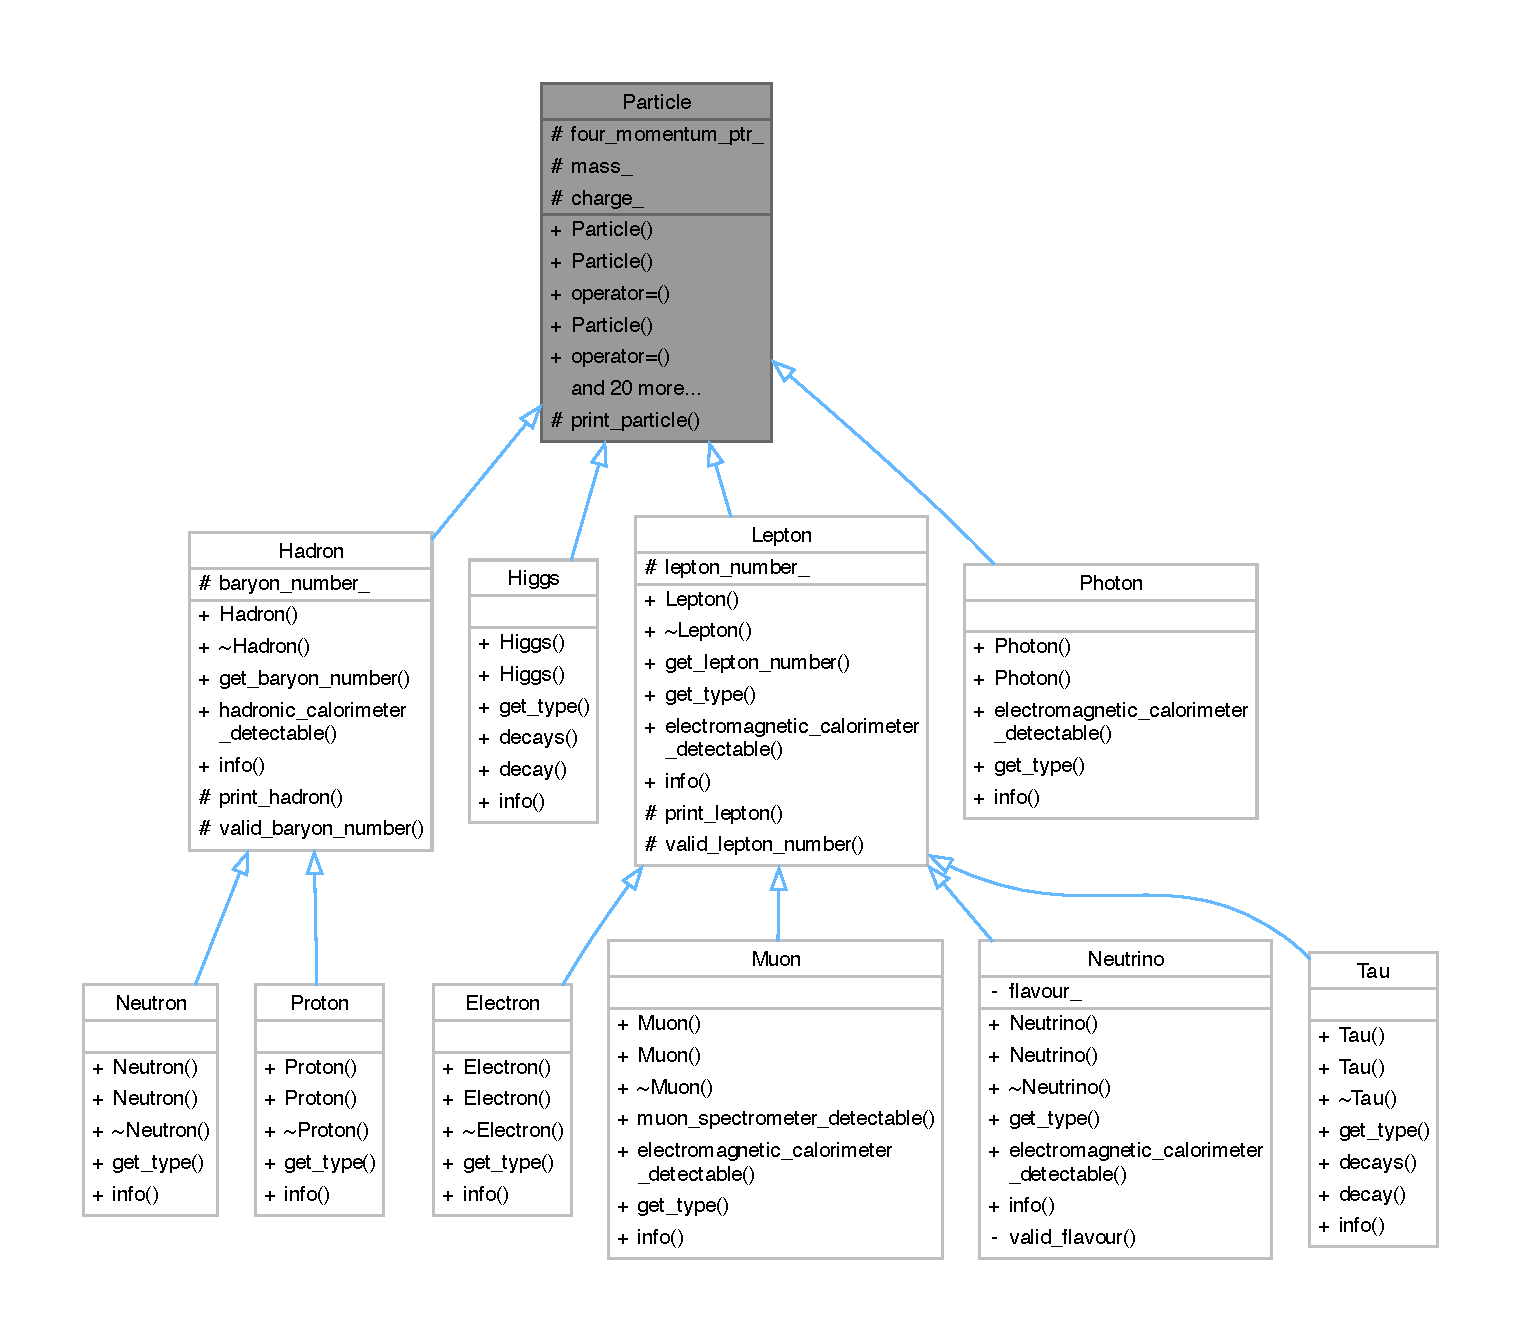
\includegraphics[scale=0.5]{class_particle__inherit__graph.pdf}
	\caption{A UML class diagram for the Particle class inheritance hierarchy. Produced by Doxygen.}	
	\label{particleuml}
\end{figure}
To create classes for the different types of particles, an inheritance hierarchy was used, shown in Figure \ref{particleuml}. For inheritance, the destructors of the parent class must be defined and virtual, and destructors defined in child class. This is so only the child class destructor is called when the object goes out of scope, avoiding double deletion.

The Particle, Hadron and Lepton classes are abstract classes, so they cannot be instantiated, but allow child classes to inherit important data members and member functions from them. Abstract classes are created by making a function within them pure virtual, using virtual keyword and an =0 at the end of the function declaration. This function must then be defined in the child class, so the info function, which prints the data about an object in this project, was used as every class must have their own defined anyway.

Non pure virtual functions were also useful, especially for flags and the decay function. The flags were boolean functions that returned true if a specific property was true for that particle, useful if it couldn't be easily discerned from another property of the particle, for example when deciding if a particle could be detected by the electromagnetic calorimeter. This was used for dynamic polymorphism in the ParticleBunch and Detector classes. 

\subsection{ParticleBunch}

The ParticleBunch class stored particles as base class unique pointers

The particle class hierarchy uses polymorphism
PLAN
OOP EXAMPLES 
encapsulation - all classes, particle probaly best
inheritance - particle hierarchy
polymorphism 
static - overloaded function - constuctors
dynamic - info() function on particles - detector flags
abstraction - particle type enum class

FEATURES USED
enum class for particle type - validation in one place
														 - easier to scale switch cases than if enables
- re used for Neutrino flavour 
deque to do particle decay
unordered map to do key value pairs 
rand() for efficiency / misdetection calulation

\section{Results}
   
\begin{lstlisting}
	int main()
	{
		return 0;
	}
\end{lstlisting} 
\section{Discussion}
errors on detected value. Extra abstraction in detect function. 
\newpage
% \bibliography{report_template_library} % Specifies the bibliography file where our references are stored. If the library file and document are not in the same folder then the file path must also be included.


\end{document}
